

\chapter*{Introducci\'on}
\pagenumbering{arabic} % para empezar la numeración con números

La produccion de papa criolla (Solanum Phureja), colombiana o yema de huevo como tambien es conocida, siempre ha tenido muchos desafios por parte de la industria, debido a los grandes intereses provenientes de los diferentes consumidores que la misma posee, siendo asi que es uno de los productos agricolas mas consumidos y con mayor importancia en el mundo, despues del arroz, maiz y trigo. Colombia es el mayor productor de papa criolla en Latinoamerica y por lo cual es un pais que posee grandes exigencias industriales de la misma (Ligarreto G - Suarez M, 2003).\\

Los tuberculos de papa criolla tienen aproximadamente entre dos y ocho centimetros (2-8cm), y se pueden clasificar en tres calibres segun su diametro promedio de donde radican los intereses comerciales de la misma. Los tuberculos de entre dos y medio y cuatro centimetros son preferidos para encurtidos y pre-cocidos mientras los tuberculos promedio entre cuatro y seis y medio centimetros son preferidos para frituras en hojuelas o con mas de cinco centimetros para frituras en tiras (CORPOICA, 2009).\\

El crecimiento vegetal es definido por Cabezas en 2005 como "`El aumento irreversible del tamaño y peso seco de las plantas (altura, área foliar, diámetro, número de células y cantidad de protoplasma) o los cambios que ocurren en una planta o población de plantas a través del tiempo, fenómeno acompañado del aumento en la complejidad estructural metabólica del organismo (diferenciación celular, número de hojas), por procesos de división y alargamiento celular, incorporación de materia y energía del ambiente (fotosíntesis, absorción de agua y de iones) y metabolización subsiguiente, la cual se traduce en multiplicación y diferenciación celular. Este proceso está íntimamente relacionado con algunos factores internos como fotosíntesis, respiración, transpiración, condiciones de estrés, concentración enzimática, balance hormonal y expresión genética"' (Pineros C, 2009).\\

En la papa son dos los procesos fisiologicos asocidos directamente al rendimiento de la misma, la fotosintesis y la respiracion. Y estos dos son procesos intimamente asociados, ya que durante la fotosintesis se producen carbohidratos que son consumidos durante la respiracion, pero una gran cantidad de estos carbohidratos contribuyen al proceso de produccion incrementando el tamano de los tuberculos, el nivel y periodo de creciemiento de los tuberculos es una variable que responde directamente a la expresion de rendimiento expresada como produccion por dia, siendo asi que cerca de un noventa por ciento (90\%) del peso acumulado de los tuberculos producidos por una planta es producto de la asimilacion de dioxido de carbono, asi como otros procesos similares (Beukema, 1979). Sin embargo, estos procesos se ven afectados por condiciones externas tales como la itensidad de luz, temperatura, longitud de los dias, condiciones del suelo que son variables no controladas, o por condiciones como la cantidad de riego, fertilizantes aplicados y productos de abono para la mejora de los suelos que son variables controlables pero que requieren de costos adicionales de produccion (Pineros C, 2009). Y es por ello que se sigue buscando con el manejo de variables controladas el control sobre la cantidad total producida y tamano de los tuberculos sin producir costos adicionales, siendo la densidad de siembra una de estas variables, en la cual nos enfocaremos en esta investigacion (Darghan E - Bernal E - Rodriguez L, 2017).\\

Las variables que influyen en el rendimiento de la papa pueden ser observados en la \ref{fig:arch}. Pag.\pageref{fig:arch}.\\
\begin{figure}[h]
	\caption{Variables de influencia sobre el rendimiento de Solanum Phureja.}
	\centering
	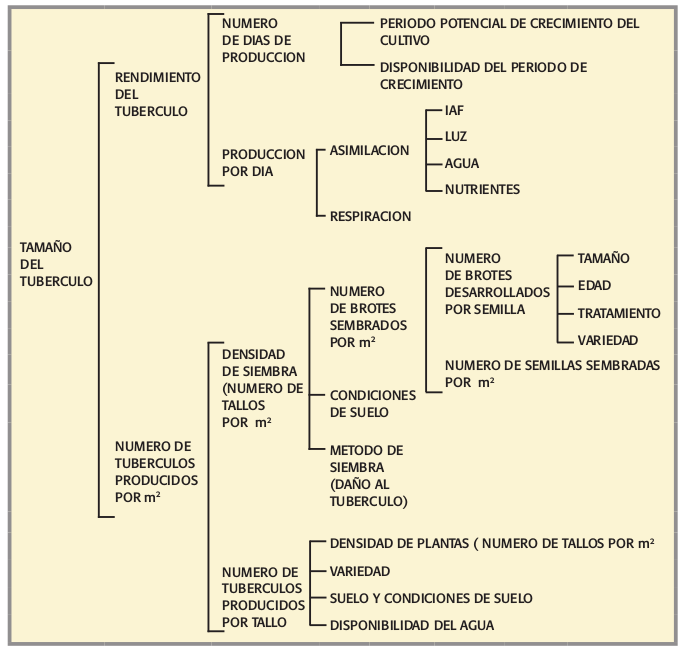
\includegraphics[scale=0.5]{variables.png}
	\label{fig:arch}
\end{figure}

Sin embargo la densidad de siembra es una variable de tipo espacial, ya que se define como la distancia entre plantas y entre linderas, siendo asi una coordenada en X y una coordenada en Y en un plano cartesiano, por lo cual un estudio estadistico de la misma para clasificar o predecir un modelo no puede ser del tipo de regresion lineal o de un analisis de varianza debido a los residuales que deben ser independientes en cada punto, no tomando en cuenta una relacion entre vecinos como si ocurre en los cultivos de papa, las plantas compiten por los recursos y por consiguiente por producir mas, haciendo asi los residuales dependientes y asi mismo no optima la aplicacion de dichos analisis (Pineros C, 2009). \\

Se plantea el uso de regresion espacial entonces, pero el manejo de la densidad de siembra como variable es del tipo cualitativo con un valor de distancia entre linderos y plantas fijo para una cantidad de densidades definidas, implicando tener que aplicar regresion espacial para cada uno de los valores de estas densidades. Sin embargo aunque estos analisis me arrojen resultados con un comportamiento y una distribucion estadistica similar, no se puede asegurar una relacion entre cada una de las densidades definidas basados en una normalizacion n-variante, donde n seria el numero de densidades definidas. Por ello se propone en esta investigacion el uso de una red neuronal probabilistica (PNN) donde no importan los supuestos y definiciones de un modelo lineal.\\

Una red neuronal artificial (ANN) es un conjunto de nodos de un programa (neuronas) interconectados entre si, simulando el proceso de pensamiento humano, se pudiera considerar como una caja negra entrenada previamente para esperar una entrada y basado en las caracteristicas o comportamiento de la misma proporcionar una determinada salida, eliminando asi la necesidad de diferentes algoritmos que deban analizar comportamientos cada uno por separado. Una red neuronal probabilistica (PNN) no es mas que una ANN que usa funciones estadisticas que escalan la variable no linealmente como una forma de campana o una distribucion normal (Stephen G, 2007).\\

El objetivo de esta investigacion es construir un clasificador de densidades de siembra a traves de una red neuronal probabilistica, ademas de comparar los resultados provenientes de una regresion espacial versus datos observados, para concluir cuan efectivo puede ser aplicar una regresion espacial para estos casos.\\